\begin{savequote}[45mm]
\ascii{Do the simplest thing that could possibly work.}
\qauthor{\ascii{- Kent Beck}}
\end{savequote}

\chapter{物理设计} 
\label{ch:physical-design}

\section{头文件}

\begin{content}

\begin{regulation}
杜绝创建巨型头文件,将所有实体声明都放到头文件中
\end{regulation}

不是所有的宏,const常量,函数声明,类定义都要放在头文件中;而是将外部真的依赖于的实体声明放到头文件。实现文件是将实现细节进行封装隐藏的一种惯用技术。

巨型头文件必然导致包含此头文件的实体产生巨大的编译时依赖,同时也阻碍了头文件进一步演进、修改、扩展的可能性。

\begin{regulation}
自定义头文件必须具有扩展名,以区分标准库的头文件;团队头文件,源文件扩展名类型必须保持一致性
\end{regulation}

\begin{table}[H]
\resizebox{0.95\textwidth}{!} {
\begin{tabular*}{1.2\textwidth}{@{}ll@{}}
\toprule
\ascii{文件类型} & \ascii{支持的扩展名} \\
\midrule
\ascii{头文件}  & \ascii{.h, .hpp, .hxx, .hh, h++, .tcc} \\
\ascii{源文件} & \ascii{.cpp, .cxx, .cc, .c++} \\ 
\bottomrule
\end{tabular*}
}
\caption{扩展名别表}
\label{tbl:file-extension}
\end{table}

\begin{regulation}
每一个头文件都应该具有独一无二的保护宏,并保持命名规则的一致性
\end{regulation}

命名规则包括两种风格:
\begin{enum}
  \eitem{\tt{INCL\_<PROJECT>\_<MODULE>\_<FILE>\_H}}
  \eitem{\ascii{IDE自动生成唯一的序列码}}
\end{enum}

第一种命名规则问题在于:当文件名重命名,或移动目录时,需要同步修改头文件保护宏;推荐使用\ascii{IDE}自动生成头文件保护宏,其更加快捷、简单、安全、有效。

正例:
\begin{leftbar}
\begin{c++}
#ifndef INCL_RNLC_DCM_RRC_CONN_REQ_HANDLER_H
#define INCL_RNLC_DCM_RRC_CONN_REQ_HANDLER_H

#endif
\end{c++}
\end{leftbar}

或使用IDE自动生成

\begin{leftbar}
\begin{c++}
#ifndef INCL_ADCM_LLL_3465_DCPOE_ACLDDDE_479_YTEY_H
#define INCL_ADCM_LLL_3465_DCPOE_ACLDDDE_479_YTEY_H

#endif
\end{c++}
\end{leftbar}

反例:
\begin{leftbar}
\begin{c++}
// 因名称太短,可能出现名字冲突
#ifndef INCL_ACTION_H
#define INCL_ACTION_H

#endif
\end{c++}
\end{leftbar}

\begin{regulation}
路径名一律使用小写、下划线或中划线风格的名称;文件名应该与程序主要实体名称相同,可以使用驼峰命名,也可以使用小写、下划线或中划线分割的名字;实现文件的名字必须和头文件保持一致;团队内保持高度一致的命名风格
\end{regulation}

正例:
\begin{leftbar}
\begin{c++}
#include "l0-infra/trans-dsl/action/SyncActionAdapter.h"
#include "ccm_cim_adpt_rnlu_component_tdd_bp0.h"
\end{c++}
\end{leftbar}

反例:
\begin{leftbar}
\begin{c++}
// 路径名使用了驼峰命名风格
#include "l0-infra/transDsl/action/SyncActionAdapter.h"
\end{c++}
\end{leftbar}

\begin{regulation}
包含头文件时,必须保持路径名、文件名大小写敏感
\end{regulation}

因为在\ascii{windows},包含头文件时,大小写不敏感,编译时检查失效,代码失去了可移植性。所以在包含头文件时必须保持文件名的大小写敏感。

假如文件名为\code{SyncActionAdapter.h, ccm\_cim\_adpt\_rnlu\_component.h}

正例:
\begin{leftbar}
\begin{c++}
#include "l0-infra/trans-dsl/action/SyncActionAdapter.h"
#include "ccm_cim_adpt_rnlu_component.h"
\end{c++}
\end{leftbar}

反例:
\begin{leftbar}
\begin{c++}
// 路径名、文件名大小写与真实物理路径、物理文件名称不符
#include "l0-infra/trans-dsl/Action/syncactionadapter.h"
#include "CCM_CIM_Adpt_Rnlu_Component_TDD_bp0.h"
\end{c++}
\end{leftbar}

\begin{regulation}
使用\tt{extern "C"},不要包括\tt{include}语句
\end{regulation}

正例:
\begin{leftbar}
\begin{c++}
#ifndef INCL_OSS_MEM_H
#define INCL_OSS_MEM_H

#include "oss_common.h"

#ifdef  __cplusplus
extern "C" {
#endif

void* OSS_alloc(size_t);
void  OSS_free(void*);

#ifdef  __cplusplus
}
#endif

#endif
\end{c++}
\end{leftbar}

反例:
\begin{leftbar}
\begin{c++}
#ifndef INCL_OSS_MEM_H
#define INCL_OSS_MEM_H

#ifdef  __cplusplus
extern "C" {
#endif

// 不应该包含在extern "C"中
#include "oss_common.h"

void* OSS_alloc(size_t);
void  OSS_free(void*);

#ifdef  __cplusplus
}
#endif

#endif
\end{c++}
\end{leftbar}

\begin{regulation}
当以\clang{}提供实现时,头文件中必须使用\tt{extern "C"}声明,以便支持\cpp{}的扩展
\end{regulation}

正例:
\begin{leftbar}
\begin{c++}
#ifndef INCL_OSS_MEM_H
#define INCL_OSS_MEM_H

#include "oss_common.h"

#ifdef  __cplusplus
extern "C" {
#endif

void* OSS_alloc(size_t);
void  OSS_free(void*);

#ifdef  __cplusplus
}
#endif

#endif
\end{c++}
\end{leftbar}

反例:
\begin{leftbar}
\begin{c++}
#ifndef INCL_OSS_MEM_H
#define INCL_OSS_MEM_H

#include "oss_common.h"

void* OSS_alloc(size_t);
void  OSS_free(void*);

#endif
\end{c++}
\end{leftbar}

\end{content}

\section{物理设计原则}

\begin{content}

\begin{principle}
自满足原则
\end{principle}

所有头文件都应该自满足的。所谓头文件自满足,即头文件自身是可编译成功的。

看一个具体的示例代码,这里定义了一个\tt{RrmSrb1AdmitAction.h}头文件。

反例:
\begin{leftbar}
\begin{c++}
#ifndef INCL_DCM_RrmSrb1AdmitAction_H
#define INCL_DCM_RrmSrb1AdmitAction_H

struct RrmSrb1AdmitAction : SyncAction
{
    OVERRIDE Status exec(const TransactionInfo&);
};

#endif
\end{c++}
\end{leftbar}

创建对应的实现文件\tt{RrmSrb1AdmitAction.cpp},并将自身头文件的进行包含,并置在实现文件的第一行,是验证头文件自满足的最佳方式。

\begin{leftbar}
\begin{c++}
#include "rrm/actions/RrmSrb1AdmitAction.h"
\end{c++}
\end{leftbar}

如上例所示,\tt{RrmSrb1AdmitAction}对父类\tt{SyncAction}存在编译时依赖,为了满足自满足原则,其自身必须包含父类的头文件。

正例:
\begin{leftbar}
\begin{c++}
#ifndef INCL_DCM_RrmSrb1AdmitAction_H
#define INCL_DCM_RrmSrb1AdmitAction_H

#include "trans-dsl/action/SyncAction.h"

struct RrmSrb1AdmitAction : SyncAction
{
    OVERRIDE Status exec(const TransactionInfo&);
};

#endif
\end{c++}
\end{leftbar}

\begin{regulation}
实现文件的第一行代码必然是包含其对应的头文件
\end{regulation}

正例:
\begin{leftbar}
\begin{c++}
// RrmSrb1AdmitAction.cpp
#include "rrm/actions/RrmSrb1AdmitAction.h"
#include "rrm/actions/RrmSrb1AdmitReq.h"
#include "rrm/actions/RrmSrb1AdmitRsp.h"
\end{c++}
\end{leftbar}

反例:
\begin{leftbar}
\begin{c++}
// RrmSrb1AdmitAction.cpp,无法验证其对应头文件的自满足性
#include "rrm/actions/RrmSrb1AdmitReq.h"
#include "rrm/actions/RrmSrb1AdmitRsp.h"
#include "rrm/actions/RrmSrb1AdmitAction.h"
\end{c++}
\end{leftbar}

\begin{principle}
单一职责
\end{principle}

这是\ascii{SRP,Single Reponsibility Priciple}在设计头文件时的一个具体运用。头文件如果包含了其它不相关的元素,则包含该头文件的所有实现文件都将被这些不相关的元素所污染,重编译将成为一件高概率的事件。

如示例代码,将\tt{RrmSrb1AdmitAction, RrmErabSetupAdmitAction}同时定义在一个头文件中,将违背该原则。

反例:
\begin{leftbar}
\begin{c++}
#ifndef INCL_DCM_RrmAdmitAction_H
#define INCL_DCM_RrmAdmitAction_H

#include "trans-dsl/action/SyncAction.h"

struct RrmSrb1AdmitAction : SyncAction
{
    OVERRIDE(Status exec(const TransactionInfo&));
};

struct RrmErabSetupAdmitAction : SyncAction
{
    OVERRIDE(Status exec(const TransactionInfo&));
};

#endif
\end{c++}
\end{leftbar}

正例:
\begin{leftbar}
\begin{c++}
// RrmSrb1AdmitAction.h
#ifndef INCL_DCM_RrmSrb1AdmitAction_H
#define INCL_DCM_RrmSrb1AdmitAction_H

#include "trans-dsl/action/SyncAction.h"

struct RrmSrb1AdmitAction : SyncAction
{
    OVERRIDE(Status exec(const TransactionInfo&));
};

#endif
\end{c++}
\end{leftbar}

\begin{leftbar}
\begin{c++}
// RrmErabSetupAdmitAction.h
#ifndef INCL_DCM_RrmErabSetupAdmitAction_H
#define INCL_DCM_RrmErabSetupAdmitAction_H

#include "trans-dsl/action/SyncAction.h"

struct RrmErabSetupAdmitAction : SyncAction
{
    OVERRIDE(Status exec(const TransactionInfo&));
};

#endif
\end{c++}
\end{leftbar}

\begin{principle}
最小依赖
\end{principle}

一个头文件只应该包含必要的实体,尤其在头文件中仅仅对实体的声明产生依赖,那么前置声明是一种有效的降低编译时依赖的技术。

反例:
\begin{leftbar}
\begin{c++}
#ifndef INCL_transaction_dsl_EventHandler_H
#define INCL_transaction_dsl_EventHandler_H

#include "base/Keywords.h"
#include "base/Status.h"
#include "fw/event/Event.h"

INTERFACE(EventHandler)
{
    ABSTRACT(Status handleEvent(const Event&));
};

#endif
\end{c++}
\end{leftbar}

如示例代码,定义了一个\tt{EventHandler}的接口,对\tt{Event}仅仅是一个声明依赖,并没有必要包含\tt{Event.h},前置声明是解开这类编译依赖的钥匙。

注意,对\tt{typedef WORD32 Status;}的依赖,以及对宏\tt{INTERFACE}定义的依赖则需要包含相应的头文件,以便实现该头文件的自满足。

正例:
\begin{leftbar}
\begin{c++}
#ifndef INCL_transaction_dsl_EventHandler_H
#define INCL_transaction_dsl_EventHandler_H

#include "base/Keywords.h"
#include "base/Status.h"

struct Event;

INTERFACE(EventHandler)
{
    ABSTRACT(Status handleEvent(const Event&));
};

#endif
\end{c++}
\end{leftbar}

在选择包含头文件或前置声明的时候,很多程序员感到迷茫。其实规则很简单,在如下场景,前置声明即可,无需包含头文件:

\begin{enum}
  \eitem{\ascii{指针}}
  \eitem{\ascii{引用}}
  \eitem{\ascii{返回值}}
  \eitem{\ascii{函数参数}}
\end{enum}

相反地,如果编译器需要知道实体的真正内容时,则必须包含头文件,此依赖也常常称为强编译时依赖。强编译时依赖主要包括如下几种场景:
\begin{enum}
  \eitem{\tt{typedef}定义的实体}
  \eitem{\ascii{继承}}
  \eitem{\ascii{宏}}
  \eitem{\tt{inline}}
  \eitem{\tt{template}}
  \eitem{\ascii{引用类内部成员时}}
  \eitem{执行\tt{sizeof}运算}  
\end{enum}

\begin{principle}
最小可见性
\end{principle}

在头文件中定义一个类时,清晰、准确的\tt{public, protected, private}是传递设计意图的指示灯。其中\tt{private}做为一种实现细节被隐藏起来,为适应未来不明确的变化提供便利的措施。

不要将所有的实体都\tt{public},这无疑是一种自杀式做法。应该以一种相反的习惯性思维,尽最大可能性将所有实体\tt{private},直到你被迫不得不这么做为止,依次放开可见性的权限。

如下例代码所示,按照\tt{public-private, function-data}依次排列类的成员,并对具有相同特征的成员归类,将大大改善类的整体布局,给读者留下清晰的设计意图。

\begin{leftbar}
\begin{c++}
#ifndef INCL_transaction_dsl_SimpleAsyncAction_H
#define INCL_transaction_dsl_SimpleAsyncAction_H

#include "trans-dsl/action/Action.h"
#include "trans-dsl/utils/EventHandlerRegistry.h"

struct SimpleAsyncAction: Action
{
   template<typename T>
   Status waitOn(const EventId eventId, T* thisPointer,
            Status (T::*handler)(const TransactionInfo&, const Event&), 
            bool forever = false)
   {
      return registry.addHandler(eventId, thisPointer, handler, forever);
   }

   Status waitUntouchEvent(const EventId eventId);

private:
   OVERRIDE(Status handleEvent(const TransactionInfo&, const Event&));
   OVERRIDE(void kill(const TransactionInfo&, const Status)); 

private:
   DEFAULT(void, doKill(const TransactionInfo&, const Status));

private:
   EventHandlerRegistry registry;
};

#endif
\end{c++}
\end{leftbar}

\begin{regulation}
所有\tt{override}的函数必然是\tt{private}的,更好地保证了按接口编程的良好设计原则
\end{regulation}

反例:
\begin{leftbar}
\begin{c++}
#ifndef INCL_transaction_dsl_SimpleAsyncAction_H
#define INCL_transaction_dsl_SimpleAsyncAction_H

#include "trans-dsl/action/Action.h"
#include "trans-dsl/utils/EventHandlerRegistry.h"

struct SimpleAsyncAction: Action
{
   template<typename T>
   Status waitOn(const EventId eventId, T* thisPointer,
            Status (T::*handler)(const TransactionInfo&, const Event&), 
            bool forever = false)
   {
      return registry.addHandler(eventId, thisPointer, handler, forever);
   }

   Status waitUntouchEvent(const EventId eventId);

   // 本应该private
   OVERRIDE(Status handleEvent(const TransactionInfo&, const Event&));
   OVERRIDE(void kill(const TransactionInfo&, const Status)); 

private:
   DEFAULT(void, doKill(const TransactionInfo&, const Status));

private:
   EventHandlerRegistry registry;
};

#endif
\end{c++}
\end{leftbar}

\end{content}

\section{Inline}

\begin{content}

\begin{regulation}
头文件中避免定义\tt{inline}函数,除非性能分析报告指出此函数是程序的关键瓶颈
\end{regulation}

\cpp{}语言将声明和实现进行分离,程序员为此不得不在头文件和实现文件中重复地对函数进行声明。这是一件痛苦的事情,驱使部分程序员直接将函数实现为\tt{inline}。

但\tt{inline}函数的代码作为一种不稳定的内部实现细节,被放置在头文件里,
其变更所导致的大面积的重新编译是个大概率事件,为改善微乎其微的函数调用性能与其相比将得不偿失。除非有相关\ascii{profiling}的测试报告,表明这部分关键的热点代码需要被放回头文件中。

让我们就像容忍头文件中宏保护符那样,也慢慢习惯\clang{}/\cpp{}天生给我们带来的这点点重复吧。

但需要注意,有两类特殊的情况,可以将实现\tt{inline}在头文件中,因为为它们创建实现文件有点累赘和麻烦。

\begin{enum}
  \eitem{\ascii{virtual析构函数}}
  \eitem{\ascii{空的virtual函数实现}}
  \eitem{\ascii{\cpp{}11的default函数}}  
\end{enum}

\begin{regulation}
实现文件中鼓励\ascii{inline}函数实现
\end{regulation}

对于在编译单元内部定义的类而言,因为它的客户数量是确定的,就是它本身。另外,由于它本来就定义在源代码文件中,因此并没有增加任何“物理耦合”。所以,对于这样的类,我们大可以将其所有函数都实现为\tt{inline}的,就像写Java代码那样,\ascii{Once \& Only Once}。

以单态类的一种实现技术为例,讲解编译时依赖的解耦与匿名命名空间的使用。(首先,应该抵制单态设计的诱惑,单态其本质是面向对象技术中全局变量的替代品。滥用单态模式,犹如滥用全局变量,是一种典型的设计坏味道。只有确定在系统中唯一存在的概念,才能使用单态模式)。

实现单态,需要对系统中唯一存在的概念进行封装;但这个概念往往具有巨大的数据结构,如果将其声明在头文件中,无疑造成很大的编译时依赖。

反例:
\begin{leftbar}
\begin{c++}
#include "base/Status.h"
#include "base/BaseTypes.h"
#include "base/Keywords.h"
#include "cell/LteCell.h"
#include <vector>

struct LteCellRepository
{
    static LteCellRepository& getInstance();

    Status add(const WORD16 cellId);
    Status release(const WORD16 cellId);
    Status modify(const WORD16 cellId);
    
private:
    typedef std::vector<LteCell> Cells;
    Cells cells;
};
\end{c++}
\end{leftbar}

受文章篇幅的所限,\tt{LteCell.h}未列出所有代码实现,但我们知道\tt{LteCell.h}拥有巨大的数据结构,上述设计导致所有包含\tt{LteCellRepository}的头文件都被\tt{LteCell.h}所间接污染。

此时,可以通过一系列措施降低编译时依赖的问题。一个直觉上解决方案就是将依赖置入到源文件中,解除对\tt{LteCellRepository.h}的编译时依赖。

正例:
\begin{leftbar}
\begin{c++}
#include "base/Status.h"
#include "base/BaseTypes.h"
#include "base/Keywords.h"

struct CellVisitor;

INTERFACE(LteCellRepository)
{
    static LteCellRepository& getInstance();

    ABSTRACT(Status add(const WORD16 cellId));
    ABSTRACT(Status release(const WORD16 cellId));
    ABSTRACT(Status modify(const WORD16 cellId));
};
\end{c++}
\end{leftbar}

其实现文件包含\tt{LteCell.h},将对其\tt{LteCell.h}控制在仅本编译单元内部。

\begin{leftbar}
\begin{c++}
#include "cell/LteCellRepository.h"
#include "cell/CellVisitor.h"
#include "cell/LteCell.h"
#include <vector>

namespace
{
    struct LteCellRepositoryImpl : LteCellRepository
    {
        OVERRIDE Status add(const WORD16 cellId)
        {
            // inline implements
        }

        OVERRIDE Status release(const WORD16 cellId)
        {
            // inline implements
        }

        OVERRIDE Status modify(const WORD16 cellId)
        {
            // inline implements
        }
    
    private:
        typedef std::vector<LteCell> Cells;
        Cells cells;
    };
}

LteCellRepository& LteCellRepository::getInstance()
{
    static LteCellRepositoryImpl inst;
    return inst;
}
\end{c++}
\end{leftbar}

此处,\tt{LteCellRepositoryImpl}类实现时,所有实现都进行\tt{inline}实现,是否真正地进行\tt{inline}就让编译器自行决定吧。

注:此处为了简化实现和举例,使用了\ascii{STL}中的\tt{std::vector}。

\begin{regulation}
实现文件中提倡使用匿名\tt{namespace}, 以避免命名冲突。
\end{regulation}

匿名\tt{namespace}的存在常常被人遗忘,但它的确是一个利器。匿名\tt{namespace}的存在,使得所有受限于编译单元内的实体拥有了明确的处所。

自此之后,所有\clang{}风格,并局限于编译单元内的\tt{static}函数和变量;以及类似\ascii{Java}中常见的\tt{private static}的提取函数将常常被匿名\tt{namespace}替代。

此刻,请记住匿名命名空间也是一种重要的信息隐藏技术。

\end{content}

\section{struct VS. class}

\begin{content}

\begin{regulation}
在类定义时,建议统一使用\tt{struct};但绝不允许混用\tt{struct, class}。
\end{regulation}

除了名字不同之外,\tt{class}和\tt{struct}唯一的差别是:默认可见性。这体现在定义和继承时。\tt{struct}在定义一个成员,或者继承时,如果不指明,则默认为\tt{public},而\tt{class}则默认为\tt{private}。

但这些都不是重点。讨厌冗余和重复的我,在定义接口和继承时,冗余\tt{public}修饰符总让人不舒服。

\begin{leftbar}
\begin{c++}
struct SelfDescribing
{
    virtual void describeTo(Description& description) const = 0;
    virtual ~SelfDescribing() {}
};

class SelfDescribing
{
public:
    virtual void describeTo(Description& description) const = 0;
    virtual ~SelfDescribing() {}
};
\end{c++}
\end{leftbar}

更重要的是,我确信“抽象”和“信息隐藏”对于软件的重要性,这促使我将\tt{public}接口总置于类的最前面成为我的首选,\tt{class}的特性正好与我的期望背道而驰\footnote{\tt{class}的特性正好适合于将数据结构捧为神物的程序员,它们常常将数据结构置于类声明的最前面。}

不管你信仰那一个流派,切忌不能混合使用\tt{class}和\tt{struct}。在大量使用前导声明的情况下,一旦一个使用\tt{struct}的类改为\tt{class},所有的前导声明都需要修改。

\begin{regulation}
定义\clang{}风格的结构体时,摒弃\tt{struct tag}命名风格。
\end{regulation}

\tt{struct tag}彻底抑制了结构体前置声明的可能性,从而阻碍了编译优化的空间。

反例:
\begin{leftbar}
\begin{c++}
typedef struct tag_Cell
{
    WORD16 wCellId;
    WORD32 dwDlArfcn;
} T_Cell;
\end{c++}
\end{leftbar}

为了兼容\clang{}\footnote{在\clang{}语言中,如果没有使用\tt{typedef},则定义一个结构体的指针,必须\tt{struct T\_Cell *pcell},而\cpp{}没有这方面的要求。},并为结构体前置声明提供便利,如下解法是最合适的。

正例:
\begin{leftbar}
\begin{c++}
typedef struct T_Cell
{
    WORD16 wCellId;
    WORD32 dwDlArfcn;
} T_Cell;
\end{c++}
\end{leftbar}

\begin{regulation}
如果性能不是关键问题,考虑使用\ascii{PIMPL}降低编译时依赖
\end{regulation}

\begin{leftbar}
\begin{c++}
struct ApiHookImpl;

struct ApiHook
{
    ApiHook(const void* api, const void* stub);
    ~ApiHook();

private:
    ApiHookImpl* This;
};
\end{c++}
\end{leftbar}

\begin{leftbar}
\begin{c++}
#include "ApiHook.h"
#include "JmpOnlyApiHook.h"

struct ApiHookImpl
{
   ApiHookImpl(const void* api, const void* stub)
     : stubHook(api, stub)
   {
   }

   JmpOnlyApiHook stubHook;
};

ApiHook::ApiHook( const void* api, const void* stub)
  : This(new ApiHookImpl(api, stub))
{
}

ApiHook::~ApiHook()
{
    delete This;
}
\end{c++}
\end{leftbar}

通过\tt{ApiHookImpl* This}的桥接,在头文件中解除了对\tt{JmpOnlyApiHook}的依赖,将其依赖控制在本编译单元内部。

\end{content}

\section{template}

\begin{content}

\begin{regulation}
当选择模板实现时,请最大限度地降低编译时依赖。
\end{regulation}

当选择模板时,不得不将其实现定义在头文件中。当编译时依赖开销非常大时,编译模板将成为一种负担。设法降低编译时依赖,不仅仅为了缩短编译时间,更重要的是为了得到一个低耦合的实现。

\begin{leftbar}
\begin{c++}
#ifndef INCL_DCM_OSS_SENDER_H
#define INCL_DCM_OSS_SENDER_H

#include "base/Status.h"
#include "Pub_TypeDef.h"
#include "Pub_Oss.h"
#include "OSS_Comm.h"
#include "Pub_CommDef.h"
#include "base/Assertions.h"

struct OssSender
{
    OssSender(const PID& pid, BYTE commType)  : pid(pid), commType(commType)
    {
    }
    
    template <typename MSG>
    Status send(WORD16 eventId, const MSG& msg)
    {
        DCM_ASSERT_TRUE(OSS_SUCCESS == OSS_SendAsynMsg(eventId, &msg, sizeof(msg), commType, (PID*)&pid);
        return DCM_SUCCESS;
    }

private:
    const PID& pid;
    BYTE commType;
};

#endif
\end{c++}
\end{leftbar}

为了实现模板函数\tt{send},将\ascii{OSS}的一些实现细节暴露到了头文件中,包含\tt{OssSender.h}的所有文件将无意识地产生了对\ascii{OSS}头文件的依赖。

提取一个私有的\tt{send}函数,并将对\ascii{OSS}的依赖移入到\tt{OssSender.cpp}中,对\tt{PID}依赖通过前置声明解除,最终实现如代码所示。

\begin{leftbar}
\begin{c++}
#ifndef INCL_DCM_OSS_SENDER_H
#define INCL_DCM_OSS_SENDER_H

#include "base/Status.h"
#include "base/BaseTypes.h"

struct PID;

struct OssSender
{
    OssSender(const PID& pid, BYTE commType)  : pid(pid), commType(commType)
    {
    }
    
    template <typename MSG>
    Status send(WORD16 eventId, const MSG& msg)
    {
        return send(eventId, (const void*)&msg, sizeof(MSG));    
    }

private:
    Status send(WORD16 eventId, const void* msg, size_t size);

private:
    const PID& pid;
    BYTE commType;
};

#endif
\end{c++}
\end{leftbar}

识别哪些与泛型相关,哪些与泛型无关的知识,并解开此类编译时依赖是\cpp{}程序员的必备之技。

\begin{regulation}
适时选择\ascii{Explicit Template Instantiated},降低模板的编译时依赖。
\end{regulation}

模板的编译时依赖存在两个基本模型:包含模型,\ascii{export}模型。\ascii{export}模型受编译技术实现的挑战,最终被\cpp{C++}11}标准放弃。

此时,似乎我们只能选择包含模型。其实,存在一种特殊的场景,是能做到降低模板编译时依赖的。

\begin{figure}
  \centering
  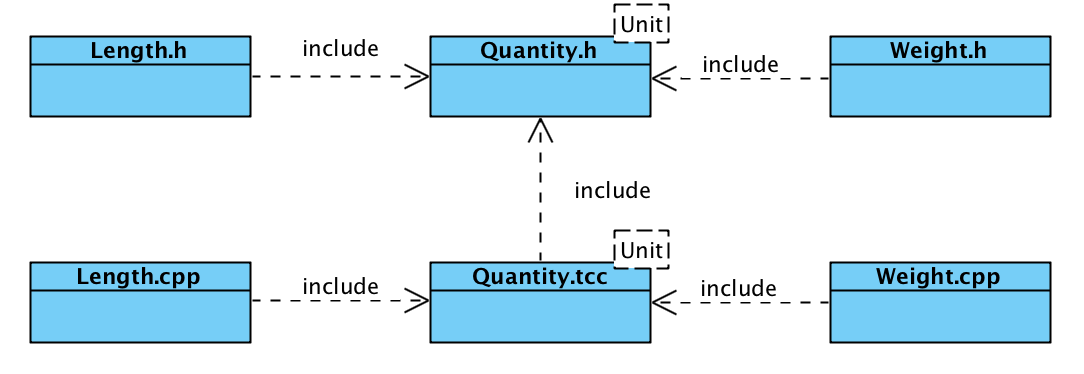
\includegraphics[width=0.8\textwidth]{figures/explict-template-inst}
  \caption{Explicit Template Instantiated}
  \label{fig:explict-template-inst}
\end{figure}

如\refig{explict-template-inst}所示,\tt{DrbSetupAdmitAction.h}仅仅对\tt{RrmAdmitAction.h}产生依赖; 特殊地,\tt{DrbSetupAdmitAction.cpp}没有产生对\tt{DrbSetupAdmitAction.h}的依赖,相反对\tt{RrmAdmitAction.tcc}产生了依赖。

当存在很多诸如\tt{DrbSetupAdmitAction.h}的子类时,编译时依赖将被彻底解除。

\begin{leftbar}
\begin{c++}
// RrmAdmitAction.h
#include "fw/action/SyncAction.h"

template <typename ADMIT_ROLE>
struct RrmAdmitAction : SyncAction
{
    OVERRIDE(Status exec(const TransactionInfo&));
};
\end{c++}
\end{leftbar}

\begin{leftbar}
\begin{c++}
// RrmAdmitAction.tcc
#include "rrm/actions/RrmAdmitAction.h"
#include "dcm_inst/UeInstanceHelper.h"
#include "cell/UeCellObject.h"
#include "base/Assertions.h"

template <typename ADMIT_ROLE>
Status RrmAdmitAction<ADMIT_ROLE>::exec(const TransactionInfo& trans)
{
    ADMIT_ROLE* role = getCurrentCell(trans);
    DCM_ASSERT_VALID_PTR(role);

    return role->admit(); 
}
\end{c++}
\end{leftbar}

\begin{leftbar}
\begin{c++}
// DrbSetupAdmitAction.h 
#include "rrm/actions/RrmAdmitAction.h"

struct RrmDrbSetupRole;

struct DrbSetupAdmitAction : RrmAdmitAction<RrmDrbSetupRole> {};
\end{c++}
\end{leftbar}

\begin{leftbar}
\begin{c++}
// DrbSetupAdmitAction.cpp
#include "rrm/role/RrmDrbSetupRole.h"
#include "rrm/actions/RrmAdmitAction.tcc"

template struct RrmAdmitAction<RrmDrbSetupRole>;

\end{c++}
\end{leftbar}

\begin{regulation}
子类化优于\tt{typedef}
\end{regulation}

\begin{leftbar}
\begin{c++}
#include "rrm/actions/RrmAdmitAction.h"

struct RrmDrbSetupRole;

struct DrbSetupAdmitAction : RrmAdmitAction<RrmDrbSetupRole> {};
\end{c++}
\end{leftbar}

这样做唯一的理由是,当仅仅出现对\tt{DrbSetupAdmitAction}的依赖时,前置声明成为可能;此外,你可以重写\tt{RrmAdmitAction}中的虚函数,实现运行时多态。

但如果实现的是\tt{typedef},除了包含头文件之外,别无他法,无疑增加了不必要的编译时依赖。

\begin{leftbar}
\begin{c++}
#include "rrm/actions/RrmAdmitAction.h"

struct RrmDrbSetupRole;

typedef RrmAdmitAction<RrmDrbSetupRole> DrbSetupAdmitAction;
\end{c++}
\end{leftbar}

\end{content}